\documentclass{supervision}
\usepackage{course}
\usepackage{float}

\Supervision{2}
\begin{document}
  \begin{questions}
    \section*{5 Constraint Satisfaction Problems}
    \question Consider the following constraint satisfaction problem:

      \begin{center}
        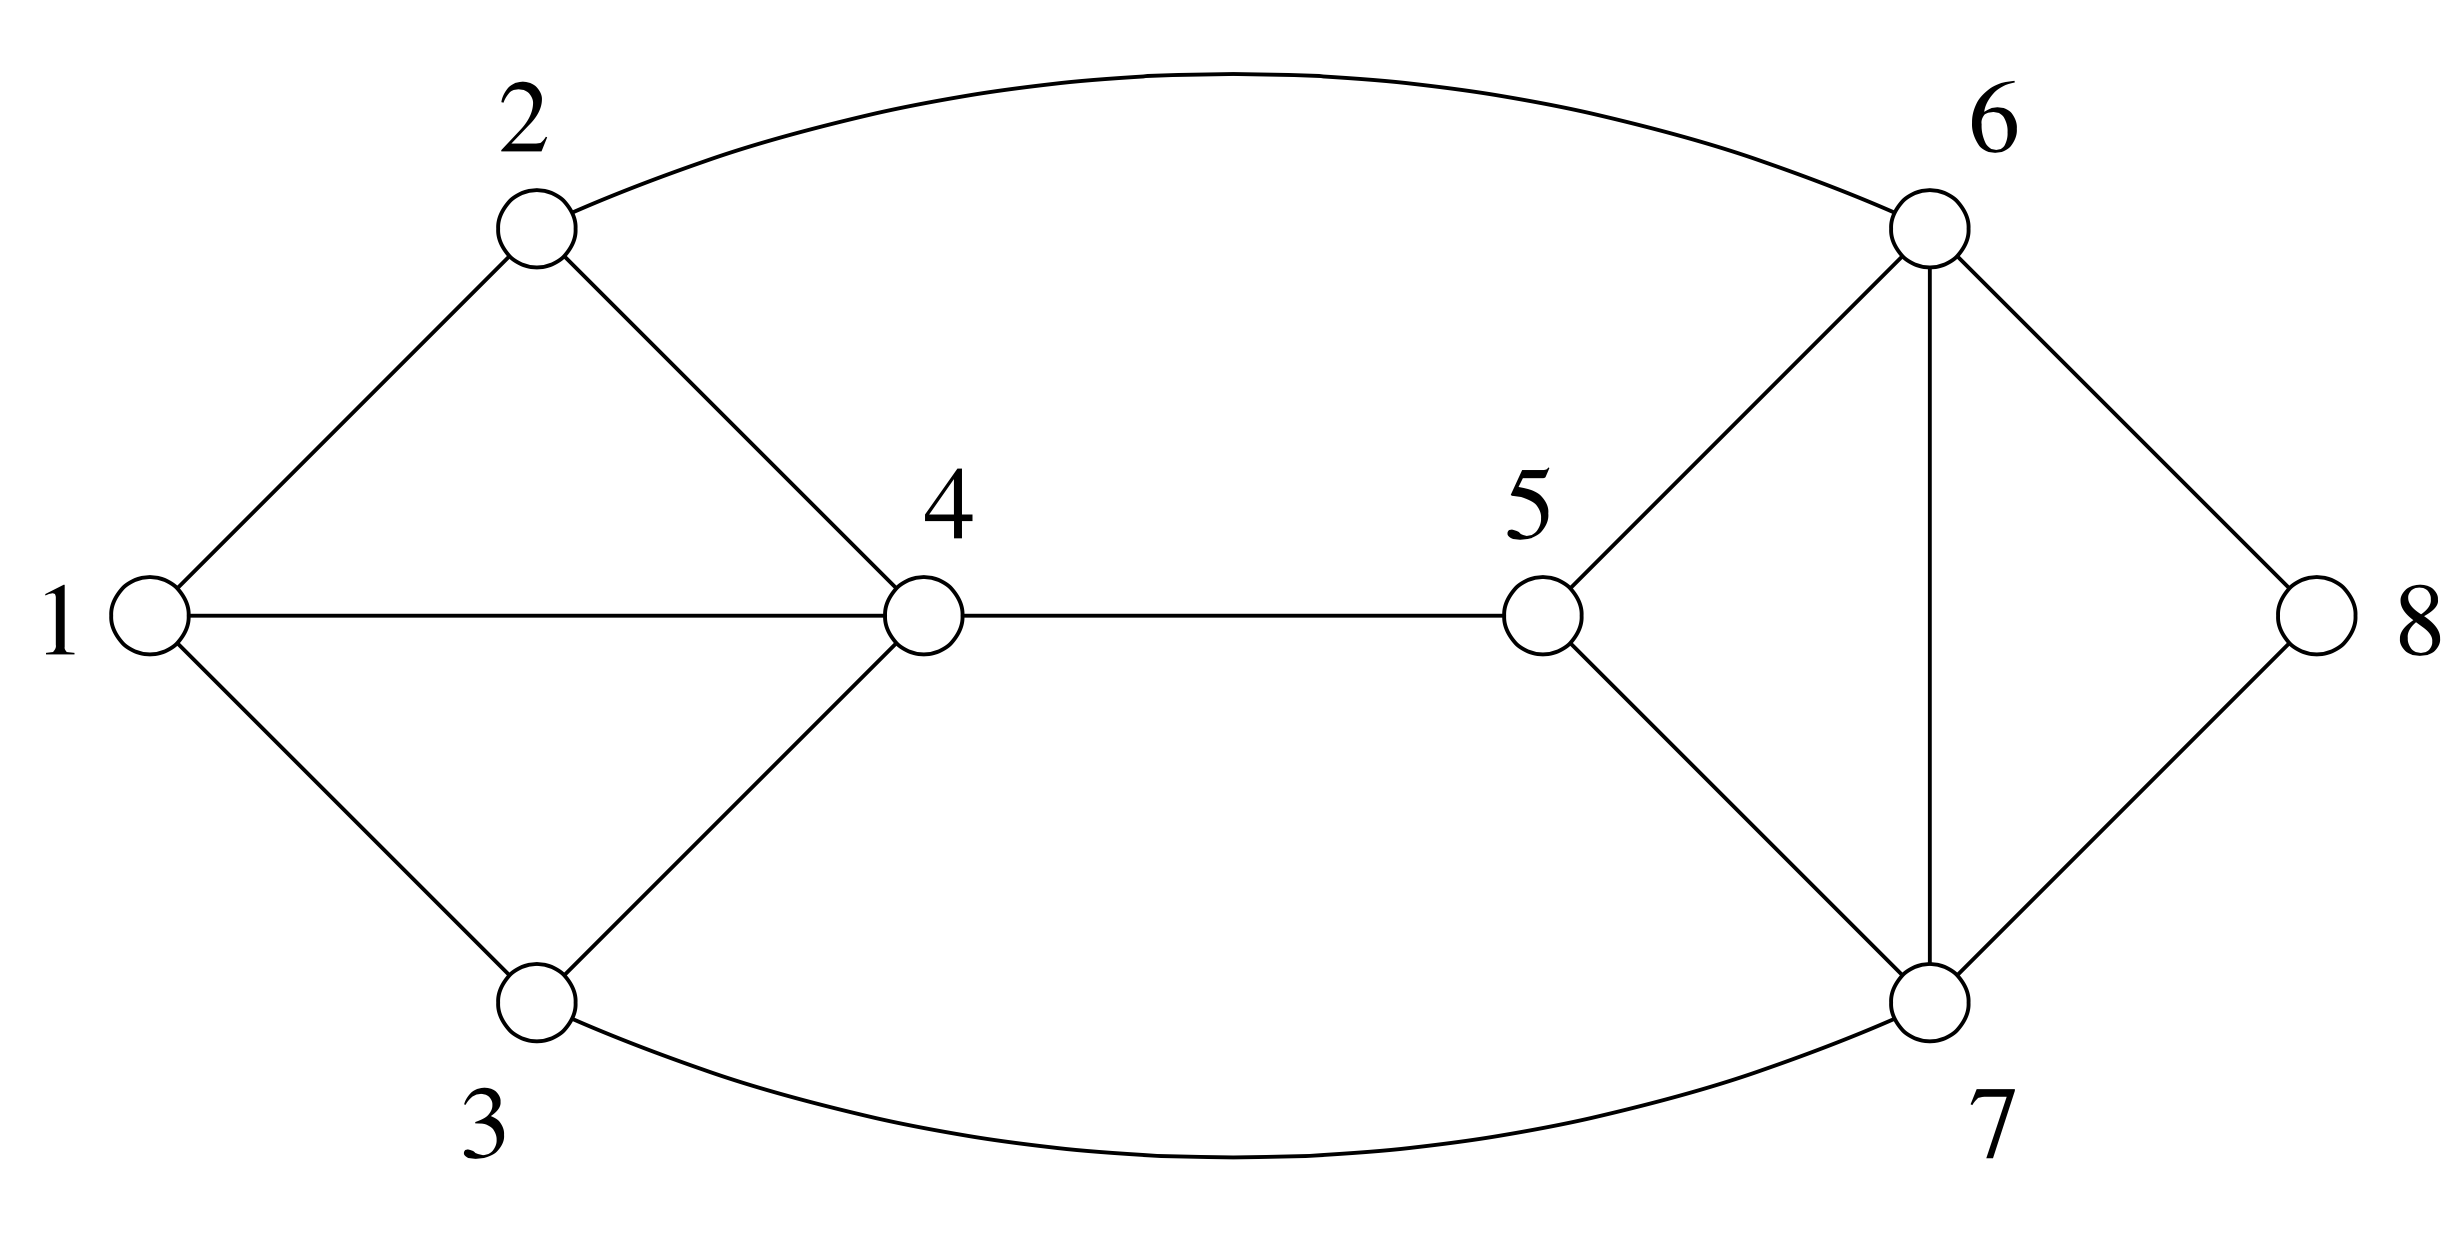
\includegraphics[width=0.7\textwidth]{2-graph}
      \end{center}

      We want to colour the nodes using the colours red (R), cyan (C) and black
      (B) in such a way that connected nodes have different colours.

      \begin{parts}
        \part Assume we attempt the assignments $1 = R$, $4 = C$, $5 = R$, $8 =
          C$, $6 = B$. Explain how forward checking operates in this example,
          and how it detects the need to backtrack.
          \begin{solution}
            \begin{table}[H]
              \begin{tabular}{|l|c|c|c|c|c|c|c|c|}
                \hline
                      & 1   & 2   & 3   & 4   & 5   & 6   & 7   & 8   \\ \hline
                START & BRC & BRC & BRC & BRC & BRC & BRC & BRC & BRC \\
                1=R   & =R  & BC  & BC  & BC  & RBC & RBC & RBC & RBC \\
                4=C   & =R  & B   & B   & =C  & RB  & RBC & RBC & RBC \\
                5=R   & =R  & B   & B   & =C  & =R  & BC  & BC  & RBC \\
                8=C   & =R  & B   & B   & =C  & =R  & B   & B   & =C  \\
                6=B   & =R  & !   & B   & =C  & =R  & =B  & !   & =C  \\ \hline
              \end{tabular}
            \end{table}
          \end{solution}

        \part Will the AC-3 algorithm detect a problem earlier in this case?
          Explain the operation of the algorithm in this example.
          \begin{solution}
            \begin{table}[H]
              \begin{tabular}{|l|c|c|c|c|c|c|c|c|}
                \hline
                      & 1   & 2   & 3   & 4   & 5   & 6   & 7   & 8   \\ \hline
                START & BRC & BRC & BRC & BRC & BRC & BRC & BRC & BRC \\
                1=R   & =R  & BC  & BC  & BC  & RBC & RBC & RBC & RBC \\
                4=C   & =R  & B   & B   & =C  & RB  & RC  & RC  & RBC \\
                5=R   & =R  & B   & B   & =C  & =R  & !   & !   & RBC \\ \hline
              \end{tabular}
            \end{table}

            As can be seen, the AC-3 algorithm has detected a problem earlier.

            When $4 = C$ is applied, the only thing remaining in the domains
            of 2 and 3 is black. The removal of cyan from these causes the
            algorithm to recheck the $6 \rightarrow 2$ and $7 \rightarrow 3$
            constraints. Black is then removed from these.

            When red is assigned to 5 it is removed from 6 and 7, leaving both
            with just cyan. This also adds the 6-7 and 7-6 constraints to be
            checked. Since they both consist of just cyan a problem is detected
            as the algorithm removes the last member of the domain.
          \end{solution}

      \end{parts}

    \section*{6 Knowledge representation and reasoning}
    \SetQuestionNumber{1}
    \question There have in fact been two queries suggested in the notes for
      obtaining a sequence of actions. The details for

      \begin{equation*}
        \exists a \exists s. {sequence}(a, s_0, s) \land {goal}(s)
      \end{equation*}

      were given on the last slide, but earlier in the notes the format

      \begin{equation*}
        \exists {actionList}.{Goal}(\ldots {actionList} \ldots)
      \end{equation*}

      was suggested. Explain how this alternative form of query might be made to
      work.
      \begin{solution}
        \emph{Not sure}
      \end{solution}

    \question Making correct use of the situation calculus, write the sentences
      in FOL required to implement the Shoot action in Wumpus World.
      \begin{solution}
        ${At}(l, s) \land {Available}({arrow}, l, s)\implies {Poss}({shoot}, s)$

        ${Poss}({shoot}, s) \implies \lnot Have({arrow}, {result}({shoot}, s))$
      \end{solution}

  \end{questions}
\end{document}
